\documentclass{article}
\usepackage[UTF8]{ctex}
\usepackage{geometry}
\usepackage{natbib}
\geometry{left=3.18cm,right=3.18cm,top=2.54cm,bottom=2.54cm}
\usepackage{graphicx}
\pagestyle{plain}	
\usepackage{setspace}
\usepackage{caption2}
\usepackage{datetime} %日期
\renewcommand{\today}{\number\year 年 \number\month 月 \number\day 日}
\renewcommand{\captionlabelfont}{\small}
\renewcommand{\captionfont}{\small}
\begin{document}

\begin{figure}
    \centering
    
\includegraphics[width=8cm]{upc.png}

    \label{figupc}
\end{figure}

	\begin{center}
		\quad \\
		\quad \\
		\heiti \fontsize{45}{17} \quad \quad \quad 
		\vskip 1.5cm
		\heiti \zihao{2} 《计算科学导论》课程总结报告
	\end{center}
	\vskip 2.0cm
		
	\begin{quotation}
% 	\begin{center}
		\doublespacing
		
        \zihao{4}\par\setlength\parindent{7em}
		\quad 

		学生姓名:\underline{\qquad  万业聪 \qquad \qquad}

		学\hspace{0.61cm} 号:\underline{\qquad 1907040120\qquad}
		
		专业班级:\underline{\qquad 本研1901 \qquad  }
		
        学\hspace{0.61cm} 院:\underline{计算机科学与技术学院}
% 	\end{center}
		\vskip 2cm
		\centering
		\begin{table}[h]
            \centering 
            \zihao{4}
            \begin{tabular}{|c|c|c|c|c|c|c|}
            % 这里的rl 与表格对应可以看到,姓名是r,右对齐的;学号是l,左对齐的;若想居中,使用c关键字。
                \hline
                课程认识 & 问题思 考 & 格式规范  & IT工具  & Latex附加  & 总分 & 评阅教师 \\
                30\% & 30\% & 20\% & 20\% & 10\% &  &  \\
                \hline
                 & & & & & &\\
                & & & & & &\\
                \hline
            \end{tabular}
        \end{table}
		\vskip 2cm
		\today
	\end{quotation}

\thispagestyle{empty}
\newpage
\setcounter{page}{1}
% 在这之前是封面,在这之后是正文
\section{引言}
经过高考后我成功的进入了理想的大学中国石油大学并且幸运的进入了自己喜欢的专业人工智能,人工智能也是计算机领域新出的分支,也是计算机专业的重要部分。其实这门课最重要的还是懂得了对计算科学这一含义的理解,并且在分组演讲的时候自己收集资料不断自己学习的过程,学会的不仅仅是课本上的知识,更是适应这一行业的学习能力。

\section{对计算科学导论这门课程的认识、体会}
计算科学这门课主要讲述了计算原理的发展过程与历史经过,并把计算机的整个历史过程及关键部分与知识进行了讲解,解释计算科学哲学、科学认识论、科学方法论、学科方法论。通过这们课我逐渐了解到了我所选择的计算机这个领域,到底什么是计算机,到底计算机的原理是什么,到底谁是图灵,图灵机是什么,它的工作原理是什么以及各种与计算相关的领域与知识。通过对这门课的学习让我了解到计算科学的基本知识,其实这也是我们高等教育的关键部分,它是不同于技校的教育的突出地方。它们仅仅是教你怎么去使用编程软件并没有理解本质,而我们却常常忽视这一重要部分,这也许是我们将来能突出的关键部分。也为我将来学习人工智能奠定了一个基础,在分组演讲时我选择了强人工智能,但在这讨论它的存在性问题很唐突,所以下面还是就我对人工智能的学习与认知过程做一下报告。\par
\subsection{人工智能基本知识}
这里我还是以弱人工智能的知识作为报告的内容,而且我以后的学习方向是人工智能,人工智能就是人工造出智能化的产品,其中最关键的问题应该是机器学习,现代大数据时代与大数据挖掘技术为机器学习提供了很好的基础。然而机器学习的一个重要的内容就是深度学习,深度学习才能真正体现机器的智能化,很明显这都是非常片面的介绍。这些学习方法都是根据人类的大脑皮层的神经结构与原理进行的模拟特别是卷积神经网络很好的模仿了大脑的表层神经网络也为智能化提供了方法。现阶段人工智能主要方向有计算机视觉与自然语言处理,和数据挖掘等。卷积等其他神经网络为他们提供了方法并且在应用中性能得到了极大的提升。\par

\subsection{机器学习}
众所周知机器学习是人工智能领域一个重要的组成部分,可以说是人工智能的核心,是使计算机具有智能的根本途径。想要学人工智能首先要知道机器学习是什么。通过了解我知道了Wikipedia对机器学习的定义machine learning is the study of algorithms and mathematical models that computer systems use to progressively improve theirperformance on a specific task .machine learning algorithms build a mathematical model of sample data ,known as "training data",in order to make predictions or decisions without being expplicitly programmed to perform the task.由此可知机器学习就是通过对现有的标签数据根据人类的学习特点来让机器学习的方法,通过训练可以拟合出一个较为完美的函数从而达到一个预测与判断的能力。\par
关于机器学习的应用我阅读了期刊论文《A machine learning approach for posture recognition based on simplified shock graph》\citep{Nooritawati2009A}对人体姿态识别是我非常感兴趣的内容。在文中主要对ANN与SVM两种基于SSG对人体姿态的识别进行比较通过实验结果证明 The application of machine learning techniques to perform classification task of human posture looks promising. 可见机器学习在人体姿态识别中发挥这重要作用,它的现实作用意义也是非常大的,所以学好机器学习是是非常关键的。
对于机器学习主要有三个分类一个是有监督的学习一个是无监督学习另一个是半监督学习。对于有监督学习就是用已知某种或某些特性的样本作为训练集,以建立一个数学模型,再用已建立的模型来预测未知样,是最常用的一种机器学习方法。是从标签化训练数据集中推断出模型的机器学习任务。通过查询我了解到监督学习的关键是从标签化的训练数据集中推断出模型机器学习任务。对于监督学习主要有分类与回归问题,下面通过一个分类的例子来体现一下我对监督学习的理解,我们最常说对字母的识别假设这里有一个数据集包含A到Z的英文字母的数据集,我们现在有一个字母,需要判定它是这26个字母中的哪一个时,这就是分类问题(只不过是一个多分类而已,每个字母一个类)。分类肯定是
有依据的,这就需要用到特征这一概念,例如,我们可以用到字母的梯度特征,角点特征,笔画特征等等。根据特征,让机器去对输入的字母进行判定,分类中概率最大的就是最终的输出结果。这是我在scdn上阅读的文章-出处(https://blog.csdn.net/feelingjun/article/details/80950564)\par
对于无监督学习我阅读了期刊论文《机器学习之无监督学习释义》\citep{wujianduxuexi}通过
阅读我了解到无监督学习主要用于发现数据中的模式,,检测数据中的异常值,而未来可能会产生通用人工智能所以它的作用还是很大的,我们上面所说的监督学习的最大问题是标记训练数据的费用,那么无监督学习(不用标记数据)的最大问 题就是它通常不能很好地工作。然而,无监督学习确实有其用途:它有助于减少数据集的维数,发现 数据的模式和结构,查找相似对象的组,以及检测数据中的异常值和其他噪声。对于无监督学习就是在不考虑具体任务的情况下学习 它们观察到的数据,从而创建自主智能。换句话说,代理是出于学习的目的而去学习。从这方面来说很有可能通过它来实现强人工智能。对于无监督学习主要有聚类问题,它要求模型查找有相似数据点的分组。目前在用的聚类算法有很多种,它们的特性往往略有不同。一般来说,聚类算法会查看数据点特征向量之间的度量或者距 离函数,然后对彼此“
接近”的特征向量进行分组。如果这些类不重叠,那么聚类算法的效果最好。\par
而对于半监督学习他的优点是非常明显的,因为在现实中以及在实际运用中我们所拥有的有标签的数据是不足的,而且获得数据需要大量的成本所以半监督学习有着非常的优势,它主要是通过少量的标签数据与大量的无标签数据来进行数据的分类学习。在无监督学习中中主要有两个基本假设一个是聚类假设另一个是流行假设(它可以更加准确的刻画局部特征)另外还有增强学习,他就是外部环境对输出只给出评价而非正确答案,学习机通过强化受奖励的动作来改善自身性能。\par
谈到了机器学习自然少不了深度学习,深度学习是机器学习领域中新的研究方向,有了它才是机器更能达到最初的智能化。为了了解深度学习我阅读了论文《deep learning》\citep{SchulzDeep}里的部分内容以及《深度学习》\citep{shenduxuexi}里的相关内容。深度学习是一类模式分析方法的统称,就具体研究内容而言,主要涉及三类方法:
(1)基于卷积运算的神经网络系统,即卷积神经网络(CNN)。 
(2)基于多层神经元的自编码神经网络,包括自编码( Auto encoder)以及近年来受到广泛关注的稀疏编码两类( Sparse Coding)。
(3)以多层自编码神经网络的方式进行预训练,进而结合鉴别信息进一步优化神经网络权值的深度置信网络(DBN)。
同时它就是通过多层处理,逐渐将初始的“低层”特征表示转化为“高层”特征表示后,用“简单模型”即可完成复杂的分类等学习任务。由此可将深度学习理解为进行“特征学习”(featurelearning)或“表示学习”(representation learning)在《深度学习》中说深度学习当前应用广泛,效果佳的就在计算机视觉和语 音识别领域。而在计算机视觉方面,卷积神经网络就是典型范例。卷积神经网络是一种特殊类型的深度前馈网络,更易于训练,并且比全接连的神经网络的泛化性能更好,由此可见卷积神经网络也是一个非常重要的内容在下一部分我再具体地结合计算机视觉与卷积神经网络谈谈我的认识。后来我又在《关于深度学习的综述与讨论》\citep{zongshu}中了解到深度学习的核心学习算法,深度学习的网络结构,深度学习理论分析以及深度学习的优化技巧,其中卷积神经网络是深度学习的一个典型模型,下面通过图形来更好地认识这种神经网络.
\makeatletter

\def\@captype{figure}

\makeatother
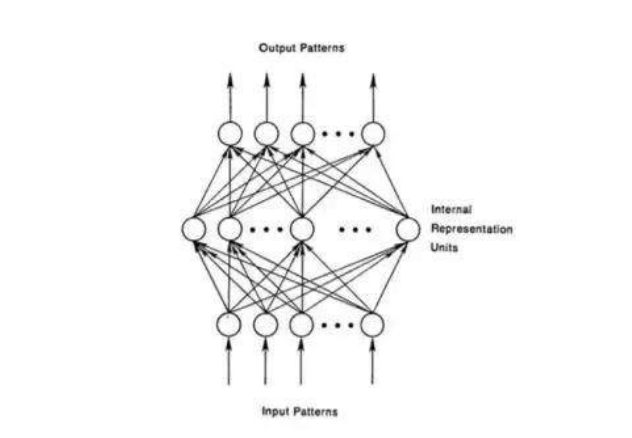
\includegraphics[scale=0.9]{juanji}
\caption{卷积神经网络模型}
\label{fig:juanjishenjingwangluo}
简单来说它主要包含三个结构,输入层,隐藏层,输出层。其实输出层中有很多个,对于cnn的隐藏层有一种基本结构卷积层+激活函数+池化层+全连接层其中卷积层的作用是进行特征提取。对于一幅输入图像,一层卷积层中包含多个卷积核,每个卷积核都能与输入图像进行卷积运算产生新的图像,新图像上的每个像素即卷积核所覆盖的一小片区域内图像的一种特征,用多个卷积核分别对图像进行卷积即可提取不同种类的特征。这也是它为什么能在计算机视觉中有如此大的优势的原因。激活函数也是非常重要的一部分它的选择对模型的性能、收敛速度都有很大的影响。对于池化层,在卷积层进行特征提取后,输出的特征图会被传递至池化层进行特征选择和信息过滤。池化层包含预设定的池化函数,其功能是将特征图中单个点的结果替换为其相邻区域的特征图统计量。池化层选取池化区域与卷积核扫描特征图步骤相同,由池化大小、步长和填充控制。卷积神经网络中的全连接层等价于传统前馈神经网络中的隐含层。全连接层位于卷积神经网络隐含层的最后部分,并只向其它全连接层传递信号。特征图在全连接层中会失去空间拓扑结构,被展开为向量并通过激励函数。这就是卷积神经网络的基本组成。\par
另一个典型的非监督学习神经网络是自编码器
\makeatletter

\def\@captype{figure}

\makeatother
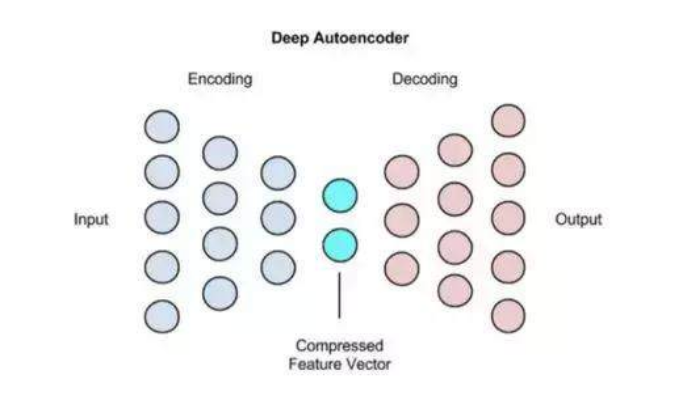
\includegraphics[scale=0.6]{zibianmaqi}
\caption{自编码器典型模型}
\label{fig:zibianmaqi}
自动编码器可以定义为由两个主要部分构成的多层神经网络。第一个部分是编码器,可以将输入数据变换成特征向量;第二个部分是解码器,可将生成的特征向量映射回输入空间。\par
\subsection{人工智能的一个方向计算机视觉}
自然计算机视觉是人工智能领域一个重要分支。计算机视觉是使用计算机及相关设备对生物视觉的一种模拟。它的主要任务就是通过对采集的图片或视频进行处理以获得相应场景的三维信息,就像人类和许多其他类生物每天所做的那样。下面我们通过一个表格了解一下计算机视觉
:\par

\begin{table}[h]
	\centering
	\caption{计算机视觉的技术与基础图}
	\begin{tabular}{r|l}
		% 这里的rl 与表格对应可以看到,姓名是r,右对齐的;学号是l,左对齐的;若想居中,使用c关键字。
		\hline
		技术 & 基础 \\
		\hline
		物体检测 & 图像处理 \\ 
		\hline
		物体识别 & 模式识别 \\
		\hline
		图像分类 & 景物分析\\
		\hline
		物体定位 & 图象理解\\
		\hline
		图像分割 & 深度学习\\
		\hline
	\end{tabular}
	\label{table1}
\end{table}
为了了解计算机视觉在现实中的应用我阅读了《A classification model of railway fasteners based on computer vision》\citep{YangA}的部分内容fastener作为railway的重要组成部分, The state of fasteners needs to be periodically checked in order to ensure safe transportation所以对它状态的判定是非常重要的,这种以计算机视觉为基础的新的识别模式打破了传统的无法识别石头下面的fasteners的局限。这让我看到计算机视觉的意义之大,让我了解到计算机视觉的应用领域是非常广的,在任何识别定位等问题上都能发挥极大的作用。这同时也让我对计算机视觉这一分支产生了极大兴趣。\par

\section{进一步的思考}
在上面我非常浅显的就弱人工智能进行了介绍,也是在分组演讲中搜集到的资料学习到的。虽然我分组演讲的主题是强人工智能,但是强人工智能在现阶段的学习上没有价值。在这次分组演讲中我毫不犹豫的选择了强人工智能,刚开始就是因为这个话题非常的火,感觉也有很多的话题可以说,所以当真正的了解到后发现并不是很简单,还有些后悔,但路都走了,总不能退回去吧,所以还是坚定的向下走了。还是认认真真的准备了这场演讲。通过这次演讲也学到很多东西。但其实最终的效果并没有达到预期的效果,完全就没有把自己的真正思想表达出来,特别是最后的提问环节完全就没有回答自己准备的资料,最后被老师怼的一败涂地,我一个对计算机知之甚少的菜鸟在老师面前显得多么的卑微,我还坚信的说在未来强人工智能一定会实现,但我知道一开始就不该说强人工智能在未来能实现,因为她根本就没有意义而且后来发现强人工智能真的不会实现。我之所以说它会实现是因为我想表达的意思在台上是根本无法表达。不是我不理解它的内涵而是当真的搜集了资料后就会发现它真的不会实现,而且它是一个未知数,我们现在所有的讨论都是没有价值的,而且种种证明都是没有价值的,对于未知的争论不是一个研究者应该做的的事情对它的研究根本就几乎不会出现有什么根本性的进步,没有什么经济价值。所以我对待强人工智能理解并不是非要证明谁是对的谁是错的,到底能不能实现。所以我真正的思考是把强人工智能作为一种方向一个目标,它不一定是去实现那个有意识,有思考的智能机器,而是以现在的弱人工智能为基础去探索现得学习方法或者神经网络去让弱人工智能更好的服务人类,就比如在自然语言处理的研究以及计算机视觉的研究它们的发展为更好地发展便利人类的生活这才是我们研究人工智能真正的目的虽然这都是弱人工智能的部分,但强与弱并不冲突。而且在未来我所研究以及学习的方向肯定还是弱人工智能的方向,学习的知识肯定还是弱人工智能,去提升弱人工智能的能力与技术让它更好的服务人类才是我们真正的目的。\par
\section{总结}
经过一学期的对计算科学的学习我最大的收获就是对计算思想的认识,这种思想在将来对计算机方面的学习与工作中作为宝贵的财富,这种思想让你在计算机领域更上一层楼。除了书本上的知识外更重要的就是我们能在实践中锻炼自己,就像分组演讲,报告,人生规划这都是我们人生中的很大锻炼,让我们成为一个综合性人才,这都是普通课程无法学到的。在这篇报告中我以弱人工智能的基本内容与我的理解做了介绍我没有对强人工智能的争辩问题进行讨论,而且最近在亚马逊的智能机器人竟然在主人问其医学知识时说出“心脏跳动是最糟糕的事情,只会消耗自然资源做出贡献。”真实原因我们也不知道。到底强人工智能会不会实现,我们谁也无法预测。或者拿谁的话或者是关系不大的研究来证明它在未来到底能不能实现,那是没有价值的,我们只有等时间来检测。所以我还是选择了在未来长期学习的弱人工智能来从中学习一些东西,在搜集资料的过程中我足步的了解了这个专业的相关知识为我也后的学习建立了一个基础。虽然我在上面介绍的内容非常片面,而且是一个初学者的视角所以有内容不专业的地方,还请老师谅解。总的来说我在整个学习过程中收获还是非常大的,感谢这门课教会了我这么多东西。\par


\section{附录}
1.github的账户。
https://wanyecong.github.io
\makeatletter

\def\@captype{figure}

\makeatother
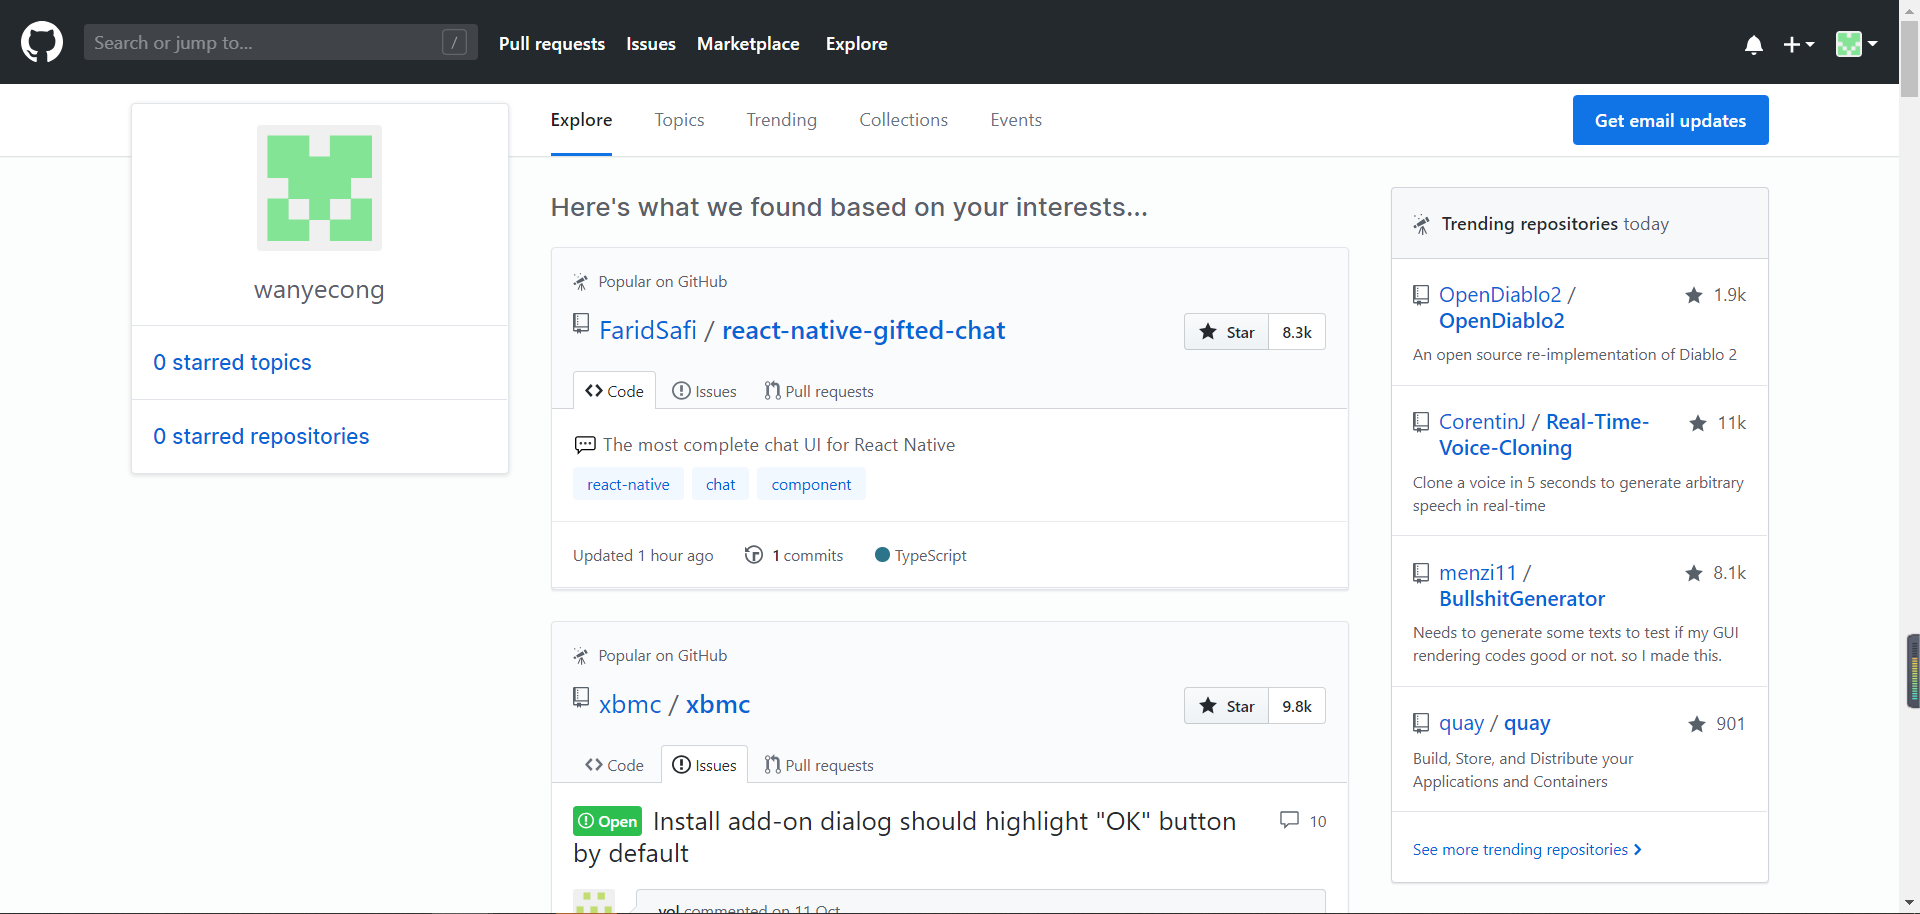
\includegraphics[scale=0.2]{github}
\caption{github账户截图}
\label{fig:github}
2.观察者
\makeatletter

\def\@captype{figure}

\makeatother
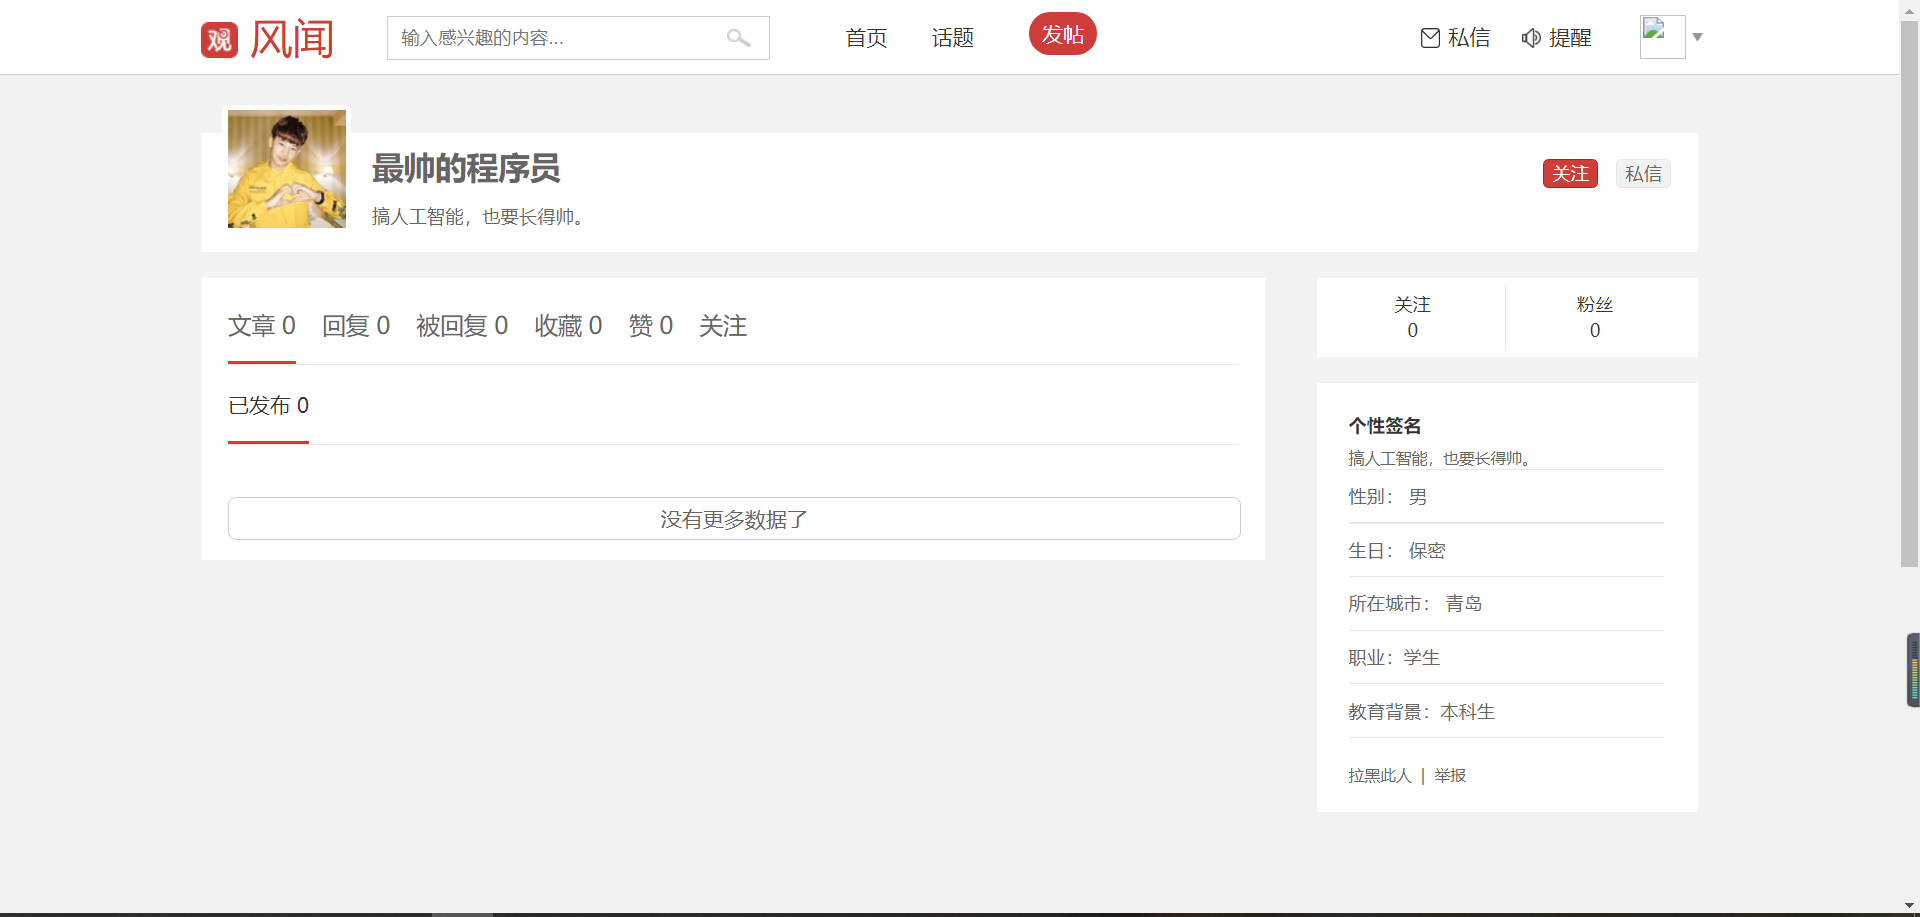
\includegraphics[scale=0.2]{guanchazhe}
\caption{观察者截图}
\label{fig:guanchazhe}
3.学习强国
\makeatletter

\def\@captype{figure}

\makeatother

\includegraphics[scale=0.1]{xuexiqiangguo}
\caption{学习强国截图}
\label{fig:xuexiqiangguo}
4.哔哩哔哩
\makeatletter

\def\@captype{figure}

\makeatother

\includegraphics[scale=0.1]{bilibili}
\caption{哔哩哔哩截图}
\label{fig:bilibili}
5.CSDN

\makeatletter

\def\@captype{figure}

\makeatother
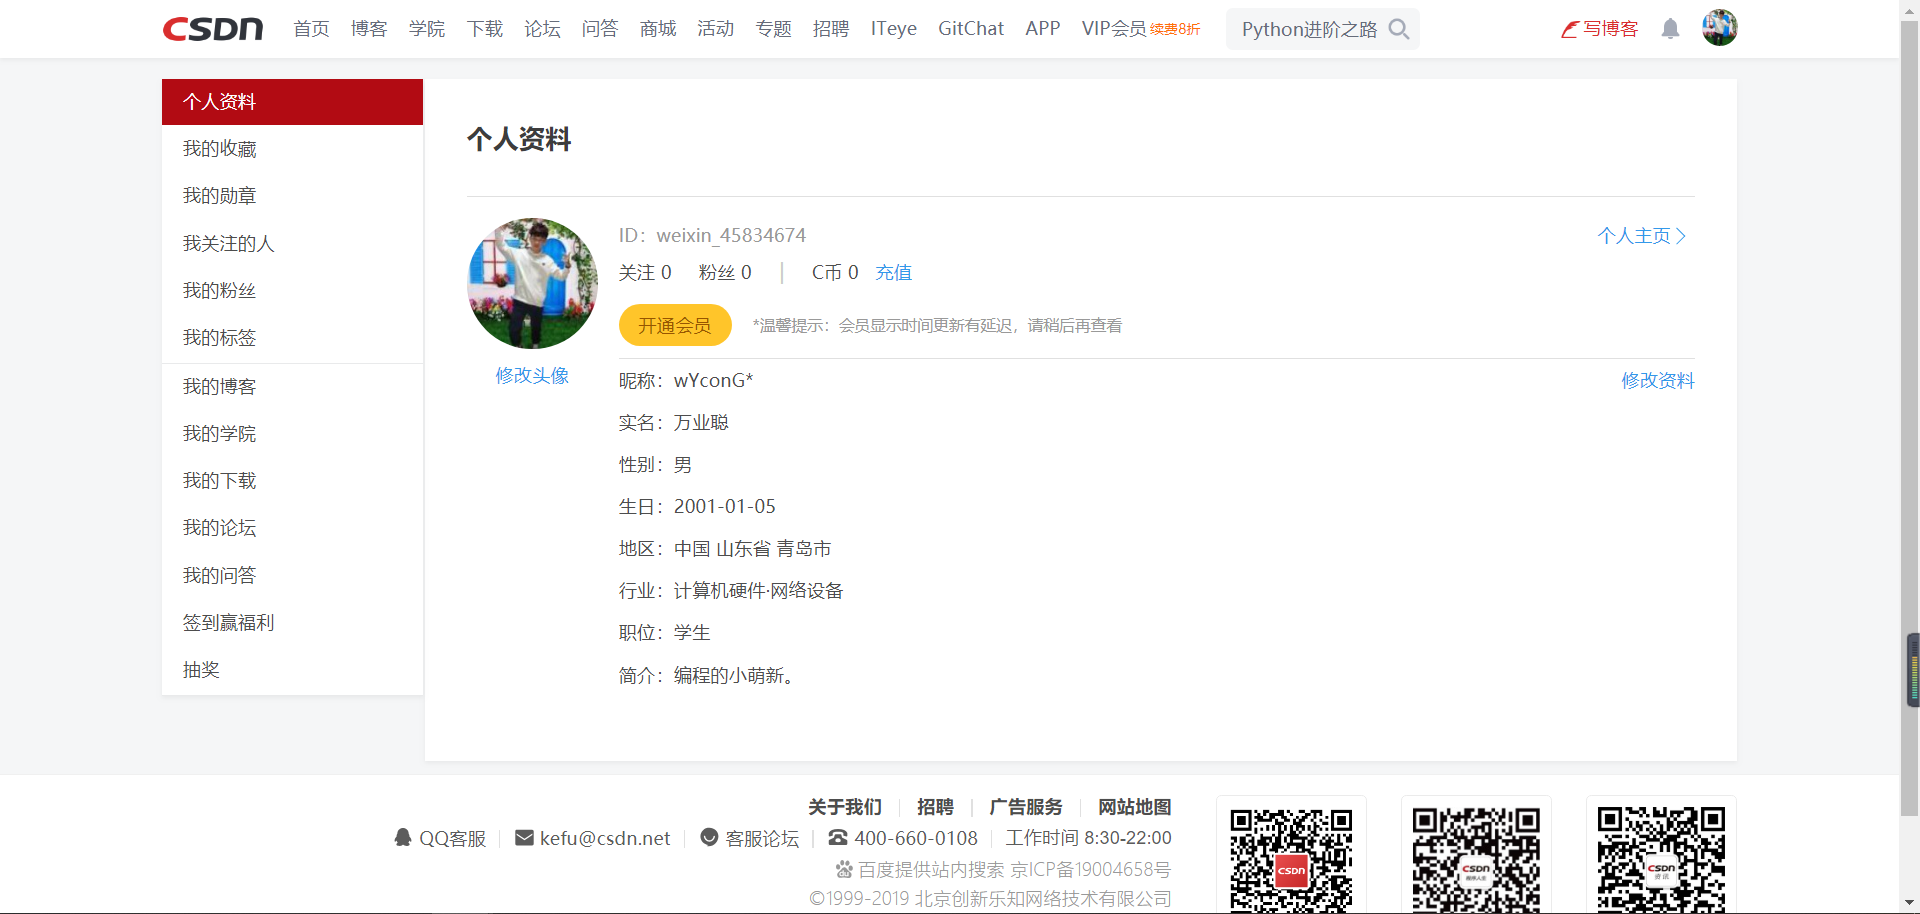
\includegraphics[scale=0.3]{csdn}
\caption{csdn截图}
\label{fig:csdn}
6.博客园
https://www.cnblogs.com/wanyecong/
\makeatletter

\def\@captype{figure}

\makeatother
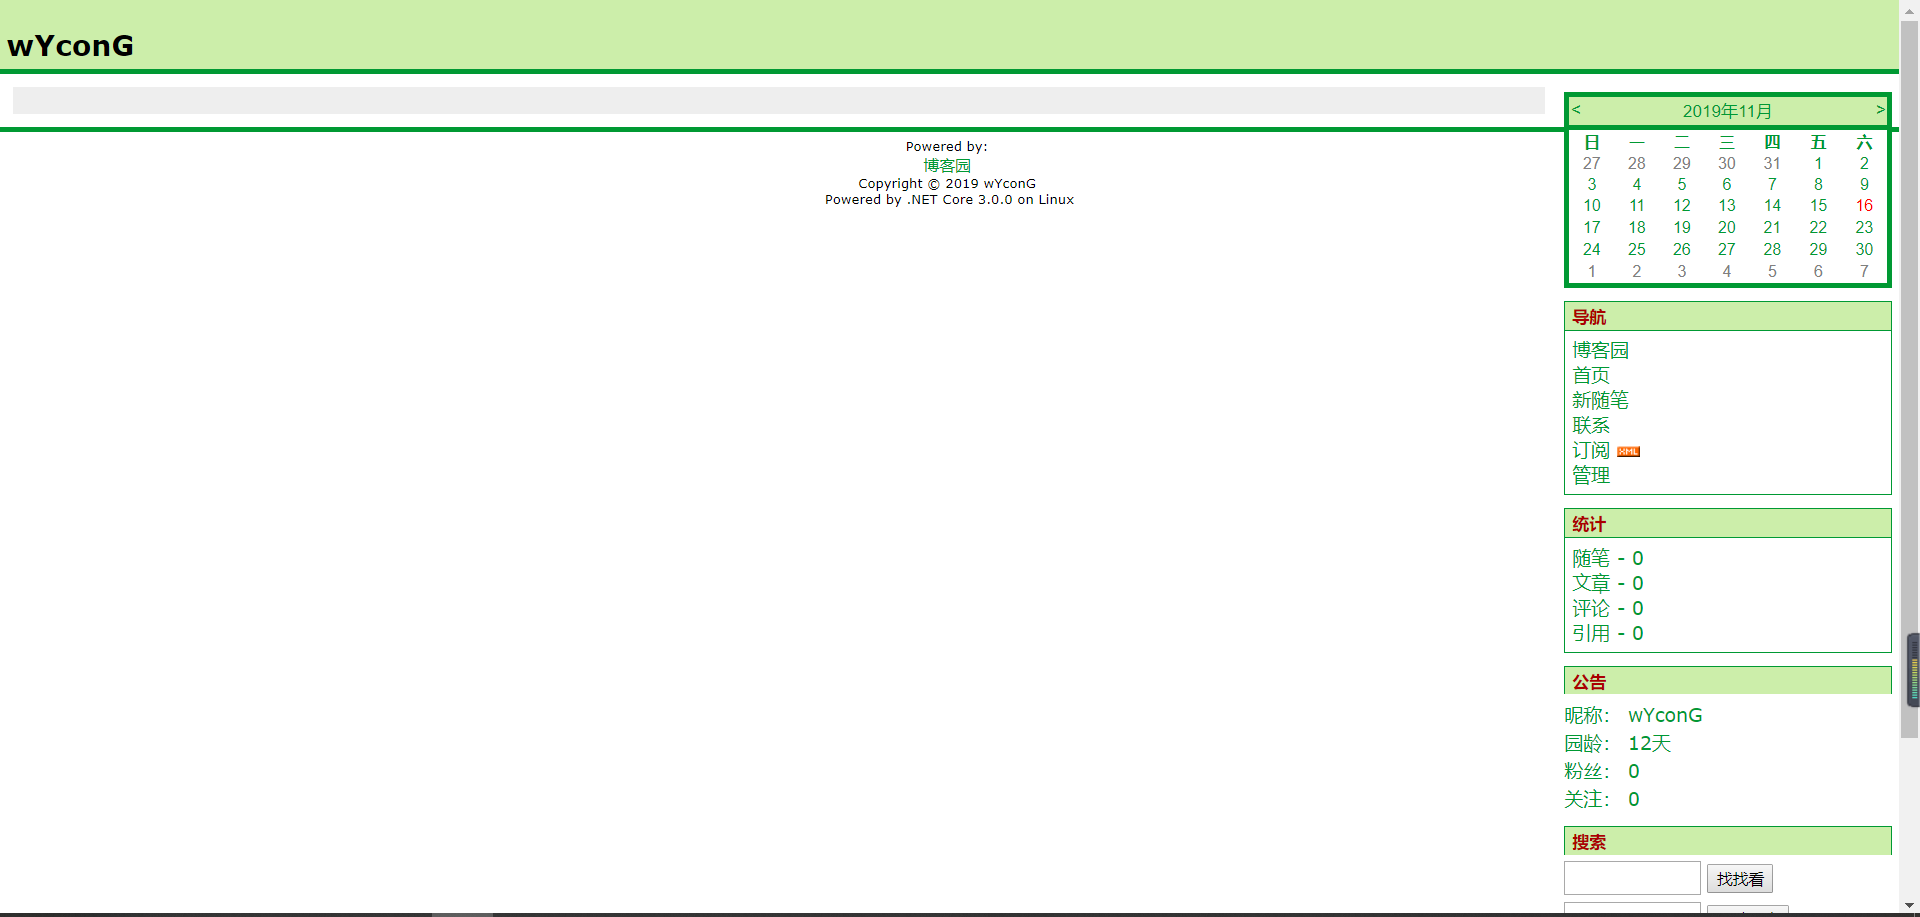
\includegraphics[scale=0.3]{bokeyuan}
\caption{博客园截图}
\label{fig:bokeyuan}

7.小木虫http://muchong.com/bbs/space.php?uid=19584345
\makeatletter

\def\@captype{figure}

\makeatother
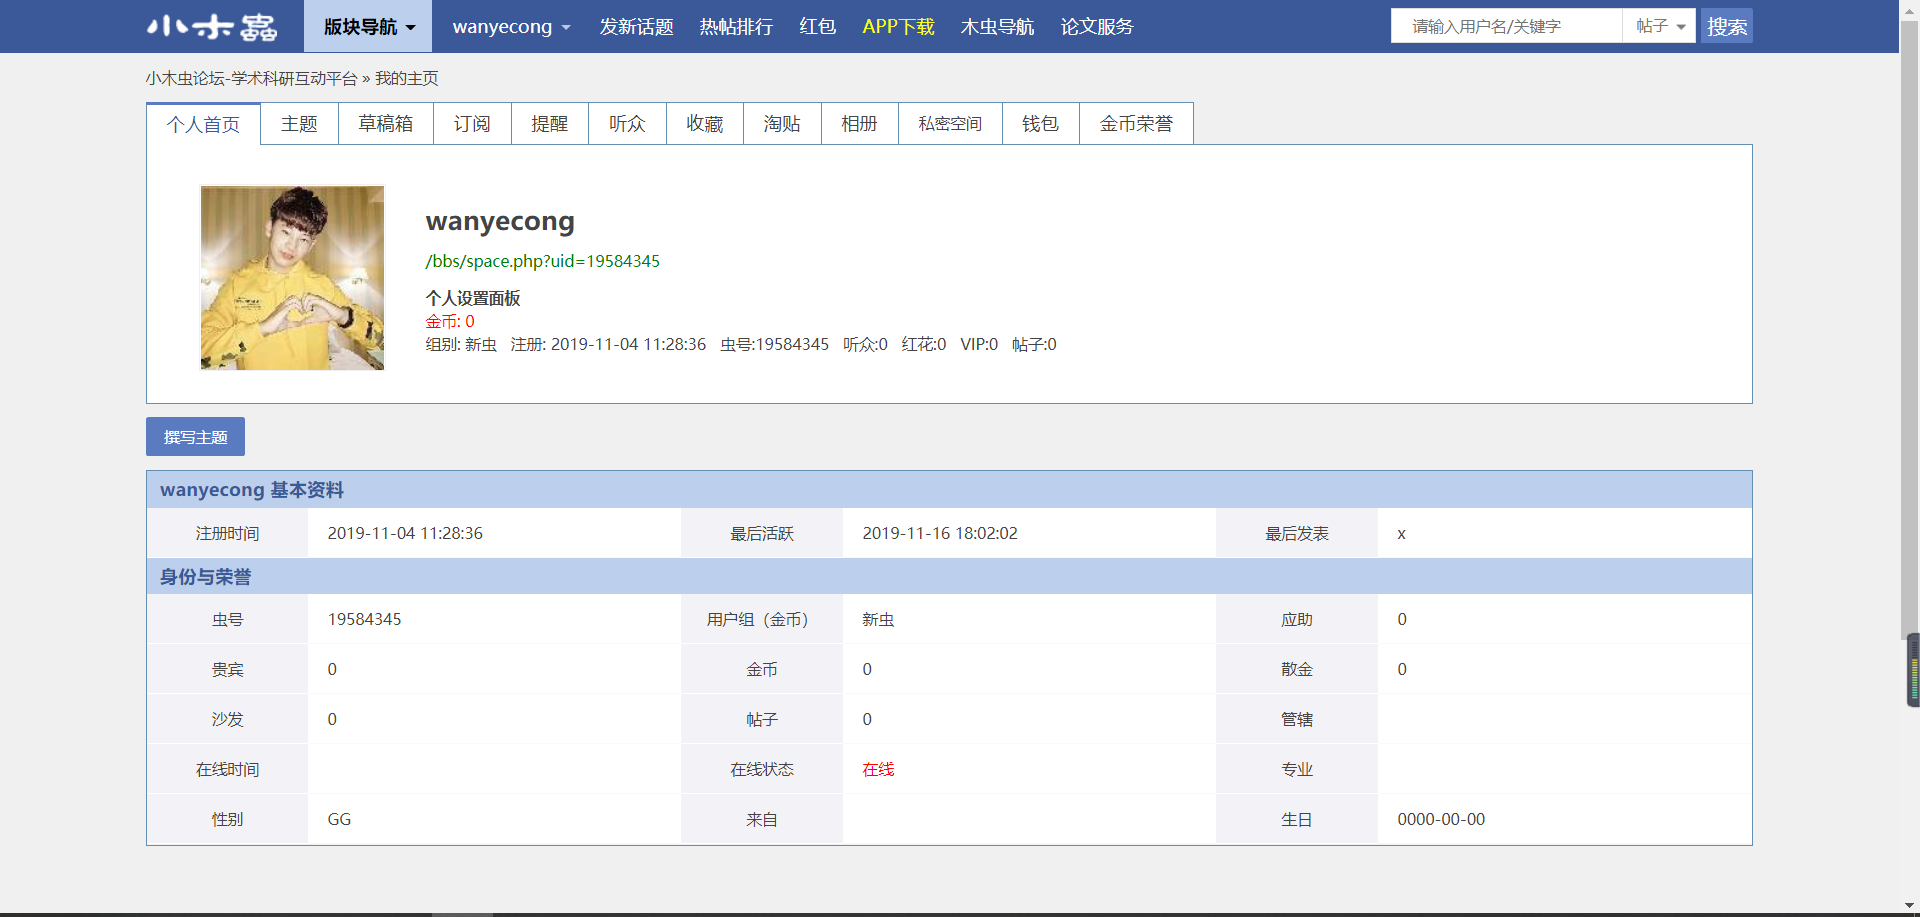
\includegraphics[scale=0.3]{xiaomuchong}
\caption{小木虫截图}
\label{fig:xiaomuchong}



\bibliographystyle{plain}
\bibliography{references}


\end{document}
